\icode{E-MD-CA-L3-261111-003}
光滑的水平面上有一木板，质量 \(M =\) \,\qty{2.0}{kg}，在木板的最右端有一小滑块（可视为质点），质量 \(m =\) \,\qty{1.0}{kg}，小滑块与木板之间的动摩擦因数 \(\mu = 0.2\)。滑块与长木板一起以 \(v_0 =\) \,\qty{2.0}{m/s}的速度向左匀速运动。如图所示，某时刻起对木板施加一个大小为\qty{12}{N}的水平向右的作用力 \(F\)，作用时间为\qty{2}{s}。小滑块始终不脱离木板。\(g\) 取\qty{10}{m/s}，试求：
\begin{enumerate}
	\item 小滑块相对地面向左运动的过程中，木板相对地面的位移；
	\item 木板长度的最小值。
\end{enumerate}

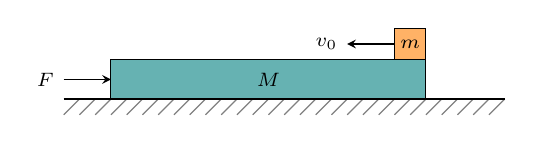
\begin{tikzpicture}[>=stealth,font=\scriptsize]
	\draw[fill=teal!60] (0,0) rectangle(4,.5)node[midway]{\(M\)};
	\draw[fill=orange!60] (3.6,.5) rectangle(4,.9)node[midway]{\(m\)};
	\draw[->] (-.6,.25)node[left]{\(F\)}--(0,.25);
	\draw[->] (3.6,.7)--++(-.6,0)node[left]{\(v_0\)};
	\foreach \x in {-.6,-.4,...,5}
		\draw[gray] (\x,-.2)--++(.2,.2);
	\draw[thick] (-.6,0)--(5,0);
\end{tikzpicture}
\begin{answer}
	（1）\qty{0.5}{m}（2）\qty{12}{m}
\end{answer}